% 1000 - 2000 words
% justify process by which the research question was answered
% justify each decision! state what each option is, why you made the choice that you did, why you rejected those not used
% justify why the chosen methods were selected as the most appropriate
% reference advantages/disadv of methods with relevance to my choice

\chapter{Methodology}

	\section{Pipeline Overview}
	
	Figure~\ref{fig:pipeline} summarises the data processing pipeline developed for finding differences in \ac{FC} between the \ac{AD}, \ac{MCI} and \ac{CS} groups. Justifications for chosen methods in different stages are found in corresponding sections.
	
	% pipeline figure here
	\begin{figure}
	    \centering
	    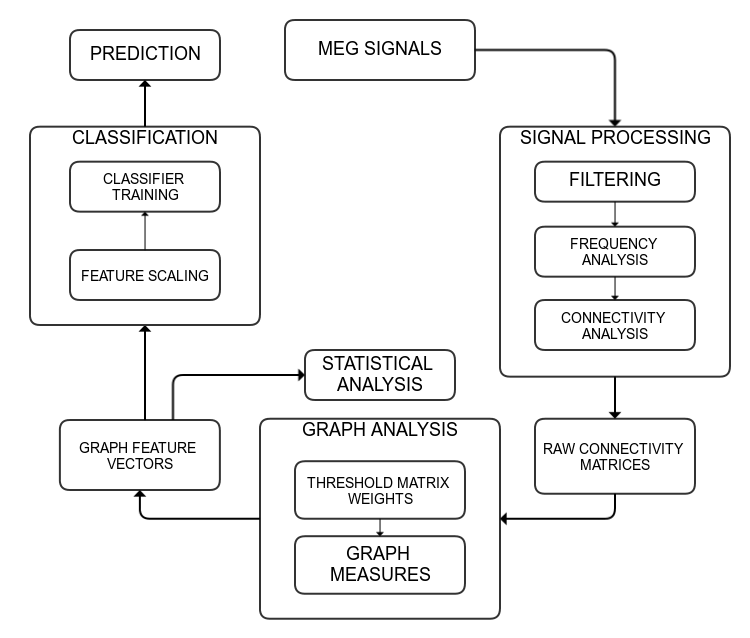
\includegraphics[width=1\textwidth]{pipeline}
	    \caption{Processing pipeline illustrating different stages of data manipulation.}
	    \label{fig:pipeline}
	\end{figure}
	%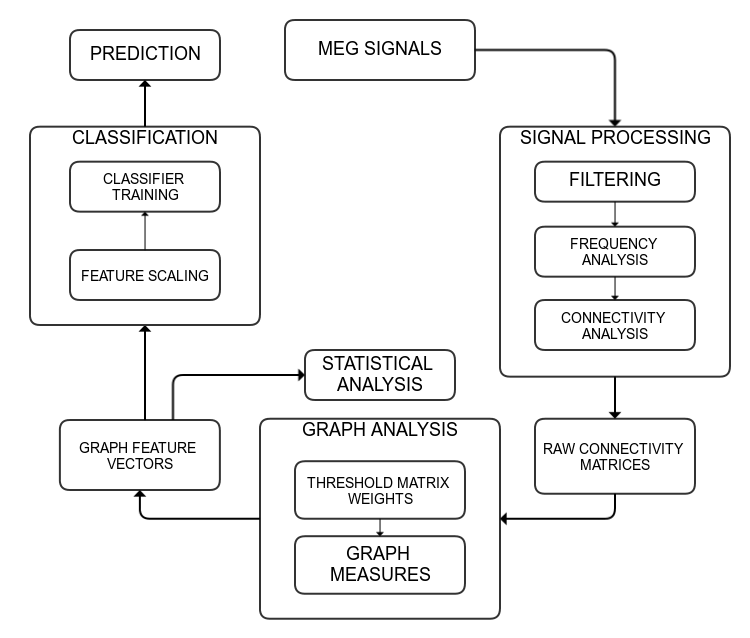
\includegraphics[scale=0.7]{pipeline.eps}

	In the signal processing stage, \ac{MEG} signals are first filtered into specific bands of interest. The frequency spectrum is then computed for these filtered signals which is then used to perform connectivity analysis between the channels. The connectivity values are saved into matrices which are then used as adjacency matrices in the graph analysis stage. Graph measures are computed from the created networks which are then combined to form feature vectors. Statistical analysis is done to verify differences between each of the \ac{CS}, \ac{MCI} and \ac{AD} groups. The graph feature vectors are finally used as training data for a number of classifiers with the goal of assigning unseen data into one of the studied groups.

	% end Overview

	\section{Dataset}
	The project made use of the same dataset employed in \textcite{Escudero2011a}. \ac{MEG} signals were recorded from a total of 80 subjects in resting-state, with their eyes closed. The data was acquired at the Centre for Biomedical Technology of the Technical University of Madrid using a 148-channel whole-head magnetometer (MAGNES 2500 WH, 4D Neuroimaging). Figure~\ref{fig:4d148} shows the layout of the 148 channels. The recordings are five minutes long, collected at a sampling frequency of 169.54 Hz. The \ac{MMSE} is a test that reflects the cognitive abilities of a subject \autocite{Folstein1975}. Such test scores have also been gathered from all participants. The number of subjects in each group, mean age with \acp{SD} and \ac{MMSE} scores can be viewed in Table~\ref{tab:dataset}.
	
	\begin{table}
		\centering
	    \begin{tabular}{llll}
	    \hline
	    Group                 & No of subjects & Mean age (\(\pm\) SD)   		 & MMSE         \\ \hline
	    CS 					  & 26             & 71.77 \(\pm\) 6.38 years                    & 28.88 \(\pm\) 1.18 \\
	    MCI                   & 18             & 74.89 \(\pm\) 5.57 years                    & 25.67 \(\pm\) 1.81 \\
	    AD                    & 36             & 74.06 \(\pm\) 6.95 years                    & 18.06 \(\pm\) 3.36   \\
	    \end{tabular}
	    \caption{Statistics of subjects used in this study}
	    \label{tab:dataset}
	\end{table}

	\begin{figure}
	    \centering
	    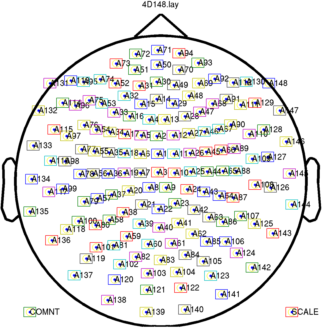
\includegraphics[width=0.7\textwidth]{4d148.png}
	    \caption{Layout of the 148 channels across the subject's head. Image from the FieldTrip toolbox \autocite{Oostenveld2011}.}
	    \label{fig:4d148}
	\end{figure}

	The provided dataset contained two sets of recordings. The first set consisted of the raw \ac{MEG} recordings which were subjected to routine preprocessing methods (see \textcite{Escudero2011a} for details), while the second set was a subset of the former and was made up of a number of 10s epoch files. These epochs were selected such that obvious ocular artefacts were not present with the help of an amplitude thresholding technique \autocite{Hornero2008}. In addition to this, the cardiac artefact was removed from these recordings with a constrained blind source separation method described in \textcite{Escudero2011b}.

	The current analysis was done on the second set of recordings cleaned of ocular and cardiac artefacts. 

	% end Dataset
	
	\section{Signal Processing} 
	
	This section describes the first part of the processing pipeline which takes as input the 10s epochs and returns connectivity matrices. Figure~\ref{fig:SPpipeline} condenses the tasks involved. The FieldTrip Matlab signal processing toolbox was used for implementation \autocite{Oostenveld2011}. A significant amount of time was spent developing this component as previous experience with signal processing was absent prior to the start of the project. 
	
		\begin{figure}
		    \centering
		    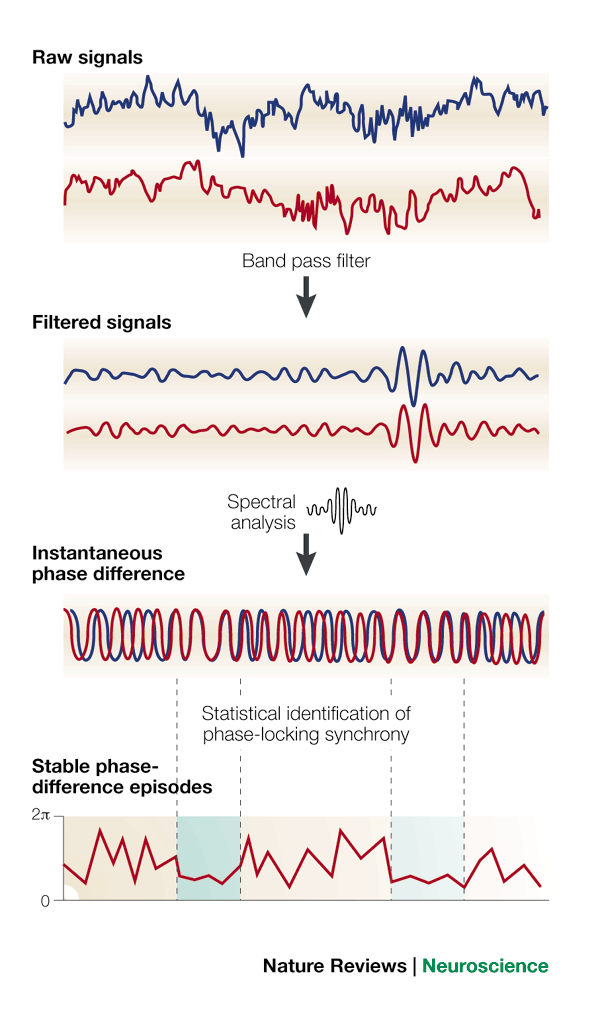
\includegraphics[width=0.7\textwidth]{phasesync}
		    \caption{Signal processing pipeline (from \textcite{Varela2001}). Raw \ac{MEG} recordings are filtered into the bands of interest. Frequency analysis is used to compute the phase of the signals. Connectivity measures employ this information to establish the level of synchronisation.}
		    \label{fig:SPpipeline}
		\end{figure}

		\subsection{Data Preprocessing}
		
		Scripts were written to check the integrity of the recordings so that invalid values or other inconsistencies across the files would not affect the next stages of the pipeline. No obvious problems were found with the given data.

				
			\subsubsection{Baseline Correction}
			It is important to note that the continuous (DC) offset is present in \ac{MEG} recordings. As it is desirable for the signals to have a variation around zero, subtraction of the mean registered value across each channel is a common preprocessing step \autocite{Gross2013}. As this is an offline analysis, the subtracted mean is computed across the whole epoch so as not to bias the mean, i.e.\ computing the mean using only the first few samples.

			\subsubsection{Filtering}
			Filtering is the process by which a signal of interest is extracted by attenuating unwanted components from the original signal \autocite{smith1997scientist}. The study aimed to inspect \ac{FC} in the following physiologically relevant bands:
			
			\begin{itemize}
				\itemsep0em
  				\item \(\delta\): 0.5 - 4 Hz  
  				\item \(\theta\): 4 - 8 Hz 	 
  				\item \(\alpha\): 8 - 13 Hz 
  				\item \(\beta\): 13 - 30 Hz 
				\item \(\gamma\): 30 - 45 Hz
			\end{itemize}

				%% ?? take it out of the text filtered epoch??
			In order to restrict connectivity analysis to a specific band, filtering was performed similarly to the study by \textcite{Stam2009}. This was done using FieldTrip's \textit{ft_preprocessing} function. Epochs were band-pass filtered for each of the above bands using a \ac{FIR} filter which effectively reduced the strength of signals outside the specified frequency intervals. An \ac{FIR} filter was chosen over an \ac{IIR} filter as the former exhibits a linear phase response whereas the latter distorts the phase of the signal \autocite{Gross2013}. Preserving the phase is crucial for correctly computing \ac{PS}. Although the filter should not in theory affect the phase, the attenuation was applied in both forward and reverse directions as an extra precaution. The filter used a Hamming window, a common and popular windowing function and a filter order of 560 to ensure that the transition from the pass to the stop band is abrupt.   

			A problem that one should be aware of is the power line interference that affects neural recordings at 50 Hz and harmonic frequencies \autocite{Keshtkaran2014}. As the highest frequency oscillations studied here are in the interval 30-45 Hz, this does not constitute a problem since the interference is high-pass filtered.

			Another problem when performing filtering is the occurrence of edge effects. These arise at the beginning and end of the epoch during the filter pass. The standard method to reduce this problem is padding the signal with extra data. A series of tests were carried out to see if padding the \ac{MEG} signals would cause a significant difference in the phases of the signals. 

			In order to better understand how the phase of a signal is obtained, the Hilbert transform is introduced in the next subsection.

		\subsection{Frequency Analysis}

			\subsubsection{Hilbert Transform}
			At the foundation of \ac{PS} measures lies the instantaneous phase. After filtering the data in a particular frequency band, the instantaneous phase at any given point in time can be extracted using the Hilbert transform \autocite{LeVanQuyen2001}. The initial time series signal \(x(t)\) can be written in analytic form as in Eq.~\ref{eq:analytic-signal}.

			\begin{equation}\label{eq:analytic-signal}
				z(t) = x(t) + i\tilde{x}(t)
			\end{equation}
			
			where \(\tilde{x}(t)\) is the Hilbert transform of \({x}(t)\):

			\begin{equation}\label{eq:hilbert-transform}
				\tilde{x}(t) = \frac{1}{\pi} p.v. \int_{-\infty}^{\infty} \frac{x({t}')}{t-{t}'}d{t'} 
			\end{equation}
			(\textit{p.v.}\ is the Cauchy principal value). The Hilbert phase is:
			
			\begin{equation}\label{eq:hilbert-phase}
				\Phi_{x}^{H}(t) = \arctan \frac{\tilde{x}(t)}{x(t)}
			\end{equation}

			Unpadded and padded signals were filtered into the bands of interest and the Hilbert transform was computed to obtain the instantaneous phase. The chosen padding was symmetric padding which follows the trend of the signal. In figure~\ref{fig:hilbert-difference} the phase difference between the padded and unpadded signals for an \(\alpha\) band filtered epoch can be observed.    

			%\input{/home/dragos/DTC/MSc/SummerProject/report/images/HilbertPhase.tex}  
			% figure: Hilbert Phase Difference
			\begin{figure}
			    \centering
			    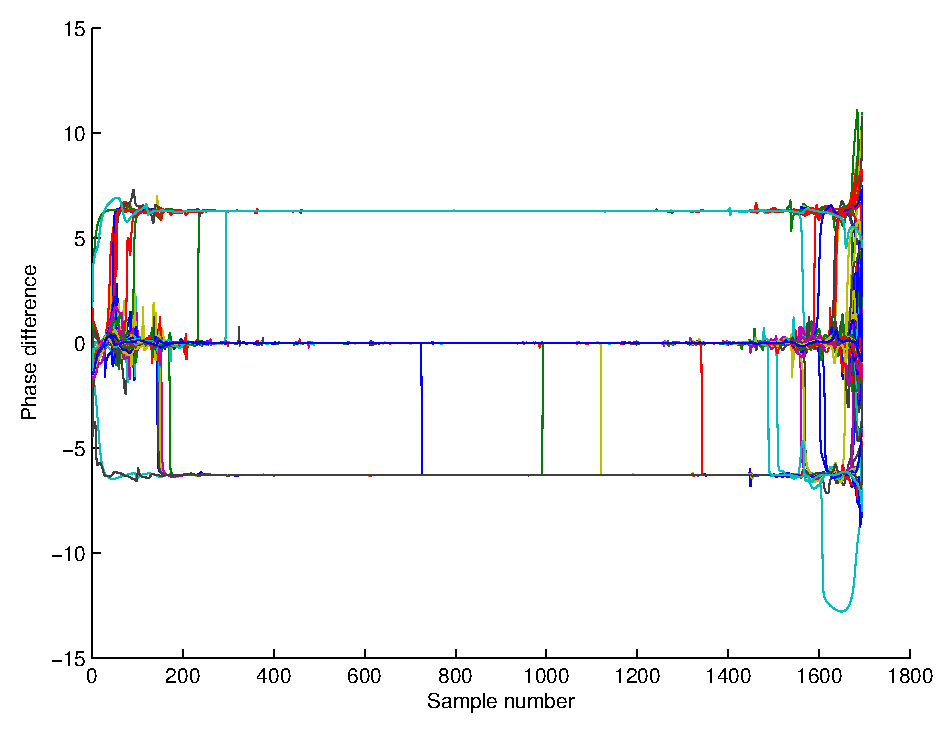
\includegraphics[width=0.8\textwidth]{HilbertPhaseDiff}
			    \caption{Subtracted phases of a padded and unpadded filtered epoch in \(\alpha\) band.}
			    \label{fig:hilbert-difference}
			\end{figure}	

			Small fluctuations of the phases occurred at the edges of the signal. This is expected because of edge effects. Visual inspection of similar phase differences in different epochs revealed similar fluctuations which were deemed insignificant to have an impact on the results. It was decided that signal padding shall not be applied.

			\subsubsection{Frequency Spectrum Estimation}
			% Welch's method and tapering	
			\ac{PS} measures require phase information which can be obtained from prior computation of the frequency spectrum. This is done by taking the Fourier transform of the given signals, which returns a series of complex numbers where the imaginary part comprises phase information. In order to reduce the amount of noise in the estimation of the frequency spectrum, Welch's periodogram method was employed \autocite{Welch1967}. The original 10s epochs were split into 2s segments with \(50\%\) overlap. These segments were then filtered into the bands of interest.

			Windowing functions, also called tapers, are multiplied with the data prior to spectral calculation to control frequency smoothing. For frequency bands below 30 Hz (\(\delta\) - \(\beta\)) it is sufficient to use only a single Hanning taper whereas for analysis in the \(\gamma\) band (30-45 Hz), multiple tapers should be used to improve frequency smoothing \autocite{Mitra1999,Percival1993}. In consequence, for the \(\gamma\) band, discrete prolate spheroidal sequences (Slepian sequences) were used as tapers with a smoothing box of \(\pm\)4 Hz \autocite{Slepian1978,Hoogenboom2006}. 

			For each 2s segment, spectral density was obtained via FieldTrip's \textit{ft_freqanalysis} function which facilitated tapering and Fourier analysis. The spectral estimates acquired in this stage were then used in connectivity analysis.

		\subsection{Connectivity Analysis}
		Connectivity measures try to quantify the degree of coupling between two signals. In the context of brain connectivity, these methods can be classified in two main categories: directed measures, which try to infer causal interactions between brain regions, and undirected measures which state the observed correlations \autocite{Friston1994}. As the goal of the project was to find differences in brain synchronisation of patients and controls during resting-state, where no particular causal interactions are sought, an undirected connectivity measure is a natural choice \autocite{Fallani2014}. The next step was to explore the available options and choose the ones most likely to yield positive results. In the past years, a series of methods were developed to address issues such as volume conduction and noise in recordings \autocite{Vindiola2014}. One of the most popular measure is the \ac{PLV} developed by \textcite{Lachaux1999} which is often used when comparing different measures \autocite{Aydore2013}. Another measure is the \ac{ImC} which is robust to spurious correlations caused by the volume conduction effect \autocite{Nolte2004}. A new measure that is gaining popularity is the \ac{dWPLI} created by \textcite{Vinck2011}. The study by \textcite{Vindiola2014} compared \ac{PLV}, \ac{ImC} and \ac{dWPLI} using simulations and found none of the measures to perform better than the others. In the present study, care was taken to develop a processing pipeline that would integrate with the FieldTrip toolbox so that different synchrony measures can be used effortlessly. This report presents the results obtained with the \ac{dWPLI} measure, but other techniques such as the \ac{PLV} and \ac{ImC} can be explored. 
		% also look at background for making this phrase cool? mention the stuff in the background at all?
			\subsubsection{Debiased Weighted Phase Lag Index}	
			The \ac{dWPLI} is an improved version of the \ac{PLI} developed by \textcite{Stam2007}. This newer technique aims to solve the problem of the \ac{PLI} not detecting changes in \ac{PS} in cases of weak coupling between the signals \autocite{Vinck2011}. It is also regarded as a method robust against volume conduction.

			\begin{equation}\label{eq:WPLI}
				{WPLI} \equiv \frac{|E\{\Im\{X\}\}|}{E\{\Im\{X\}\}} = \frac{|E\{|\Im\{X\}|sgn(\Im\{X\})\}|}{E\{|\Im\{X\}|\}}
			\end{equation}

			where \(\Im\{X\}\) is the imaginary component of the cross-spectrum between two signals \(x(t)\) and \(y(t)\). This measure returns values between 0 and 1, where 0 denotes no synchronisation and 1 indicates synchronisation. The debiased method was used in this study \autocite{Vinck2011}. Connectivity between each channel was computed using FieldTrips's \textit{ft_connectivityanalysis} function.


			% in figure the distribution of mean dWPLI values for each subject class are shown 

			%\begin{figure}
	    	%	\centering
	   		%	\includegraphics[width=0.8\textwidth]{dWPLIdistrib}
	   		%	\caption{Distribution of \ac{dWPLI} values. Mean values across subjects of each group are shown.}
	   		% \label{fig:dWPLIdistrib}
			%\end{figure}

			% distribution similar to Ortiz2012! so we can proceed to the next stage.   
			% ?? figure - histogram of dWPLI values 

		 The spectral density estimates computed in the frequency analysis step were used to calculate the connectivity values between all pairs of channels. As the recordings were made with a 148-channel \ac{MEG} machine, a \(148\times148\) matrix was computed illustrating the connectivity strength between each pair. A cell of this matrix corresponded to the correlation between the channel of the row and the channel of the column on which the cell was located. Employing Welch's method, intermediate connectivity values were computed for each 10s epoch. The final connectivity matrix of a subject was obtained by averaging the intermediate connectivity matrices across all epochs of a subject. Since the analysis was done for five bands of interest, five connectivity matrices were acquired for each subject. The matrices were then sent to the Graph Analysis module. 

	% end Signal Processing

	\section{Graph Analysis}

	This section describes the second part of the processing pipeline which takes as input the connectivity matrices from the signal processing unit and returns graph measures corresponding to the observed connectivity.

		\subsection{Constructing Brain Graphs}
		% absolute value because fieldtrip also returned negative connectivity values
		The \ac{dWPLI} connectivity matrices can be regarded as adjacency matrices of graphs modelling the subject's brain network activity for different frequency bands. Each \ac{MEG} channel can be seen as a node in the brain network, whereas entries in the matrix correspond to the strength between the nodes. For convenience, the connectivity matrix obtained in the previous stage can be written as \(W_{N \times N}\), where \textit{W} is a weighted symmetric matrix since \ac{dWPLI} is an undirected \ac{FC} metric. Although there is currently no optimal way of converting functional imaging data to graphs \autocite{StamReijneveld2007}, previous studies have consolidated certain procedures that one should take into account. 

		In the first instance, it was noticed that some negative values were obtained in the \ac{dWPLI} matrices. Consulting FieldTrip's documentation, this was normal as negative values denote anticorrelations between signals. The negative entries were replaced by their absolute values, as \textcite{Fallani2014} advise. The second step was to filter weak links as environmental noise or volume conduction may generate false correlations \autocite{Fallani2014}. A threshold \textit{X} must be chosen for deciding if an entry \(w_{ij}\) in \textit{W} is to be removed or kept. This threshold can either be an absolute threshold or a density threshold also called proportional threshold \autocite{Bullmore2011}. In the case of a simple absolute threshold, an arbitrary value is chosen which would remove edges when \(w_{ij}\) is smaller than that value. This is inappropriate as analysis would be restricted for that specific threshold \autocite{Bullmore2009}. Using a density threshold, only the top \textit{X\%} strongest links within the matrix are preserved. A varying density threshold has higher chances of finding topological differences between the networks in the three groups of interest. Care should be taken when choosing threshold values as filtering all links or keeping most of them would result in worthless analysis \autocite{Achard2007}. The five density thresholds chosen for \textit{X} are the following:

		\begin{equation}\label{eq:thresholds}
			X = \{0.05, 0.1, 0.15, 0.2, 0.3\}
		\end{equation}

		Thresholding each of the five frequency band connectivity matrices for five values produced 25 adjacency matrices per subject. A total of 2000 matrices were obtained as there are 80 subjects in the dataset.  
		Binarisation of the graphs is the step by which links that survived the thresholding process are set to unity and links that need to be removed are set to zero. The resulting matrices are treated as adjacency matrices for binary undirected graphs, where nodes \textit{i} and \textit{j} are connected if the \(w_{ij}\) entry is one. The motivation behind this step is that most graph measures used in the next stage operate only on binary graphs \autocite{Rubinov2010}.  

		\subsection{Graph Measures}

		Five graph features were calculated for each of the 25 brain graphs of a subject. The \ac{BCT} was used to compute these metrics \autocite{Rubinov2010}. Similar to the study by \textcite{Rudie2012}, the chosen measures for this step were global metrics. 

		\begin{description}
			  \item[average clustering coefficient (C)] \hfill \\
			  The local clustering coefficient of a node measures how densely connected is a node relative to the node's neighbours \autocite{Watts1998}.

			  \begin{equation}\label{eq:local-clust}
				C_i = \frac{2 e_i}{k_{i}(k_{i}-1)}
			  \end{equation}
			  where \(k_i\) is the number of neighbours of node \textit{i} and \(e_i\) is the number of edges between all of \textit{i}'s neighbours.

			  The \ac{C} is the sum of the local clustering coefficients divided by the total number of vertices. 
			  \begin{equation}\label{eq:avg-clust}
				\overline{C} = \frac{1}{n} \sum\limits_{i=1}^n C_i
			  \end{equation}
			  
			  \item[characteristic path length (L)] \hfill \\
			  \ac{L} is the average number of links in the shortest paths between every node pair in the graph.
			  \begin{equation}\label{eq:char-path-len}
				L = \frac{1}{n (n-1)} \sum\limits_{i\not=j} d(v_i, v_j)
			  \end{equation} 
			  where \(d(v_1, v_2)\) is the shortest distance between node \(v_1\) and  node \(v_2\).

			  \item[global efficiency (GE)] \hfill \\
			  \ac{GE} is the average inverse shortest path \autocite{Latora2001}. It is used instead of \ac{L} when networks have disconnected nodes \autocite{Fallani2014}.
			  \begin{equation}\label{eq:ge}
				GE = \frac{1}{n (n-1)} \sum\limits_{i\not=j} d(v_i, v_j)^{-1}
			  \end{equation} 
			  
			  \item[small-worldness (SW)] \hfill \\
			  The \ac{SW} index of a graph is defined as follows \autocite{Watts1998}:
			  \begin{equation}\label{eq:sw}		
				SW = \frac{ \frac{C}{ C_{rand} } }{ \frac{L}{ L_{rand} } }
			  \end{equation}
			  where \(C_{rand}\) and \(L_{rand}\) are the \ac{C} and \ac{L} of a random network.

			  Following the methodology described in \textcite{Rudie2012}, for each adjacency matrix, the computation of the \ac{SW} value was performed by generating a number of random networks that respected the number of nodes, node degree and edge distribution of the given adjacency matrix. In the referenced study, 100 random networks were generated for each subject network by disconnecting and randomly rewiring each edge of the given network using \ac{BCT}'s \textit{randmio_und_connected} function. The same method was applied in this study, with the observation that six random networks were generated for each matrix because of available computational resources. The average \ac{C} and \ac{L} of the created random networks became \(C_{rand}\) and \(L_{rand}\) in Eq.~\ref{eq:sw}. It is important to note that the \textit{randmio_und_connected} function, as the name suggests, maintains the connectedness property of the input graph. A connected graph is a graph where there is a path from any node to any other node.     

			  \item[modularity (Q)] \hfill \\
			  \ac{Q} quantifies to what extent can a network be divided into clearly separated clusters of nodes \autocite{Newman2003}.
			  \begin{equation}\label{eq:q}		
				Q = \sum\limits_{u \in M} \left[ e_{uu} - \left(\sum\limits_{v \in M} e_{uv} \right)^2 \right]
			  \end{equation}
			  where the graph is divided into nonoverlapping modules \textit{M} and \(e_{uv}\) is the proportion of edges connecting vertices in module \textit{u} with vertices in module \textit{v} \autocite{Rubinov2010}. 
			  For computing this measure, the \ac{BCT} \textit{modularity_und} function was used. For each graph, the function was executed 100 times as the \ac{Q} measure employs heuristics which can vary from run to run. The average of the 100 runs was taken as the final \ac{Q} for that graph.
		\end{description}

		After this stage, graph features have been computed for each subject, for all thresholds in Eq.~\ref{eq:thresholds}, for each frequency band of interest. 

	% end Graph Analysis

	\section{Statistical Testing}
	This section describes the statistical significance methods used to compare network measures between the groups.
		
		\subsection{Functional Data Analysis}
			The study by \textcite{Bassett2012} proposed \ac{FDA} to examine differences between schizophrenia patients and healthy controls. \ac{FDA} is a subfield of statistics used for curve comparison \autocite{Ramsay2005}. Each network measure computed in the previous section can be plotted as a curve, where the \textit{x} axis is the threshold value and the \textit{y} axis represent the value of the metric. 

			For between group comparisons, the nonparametric permutation test within \ac{FDA} can be used as follows: for each network measure, the average curves of \ac{AD}, \ac{MCI} and \ac{CS} groups are computed separately. Two groups, for example \ac{AD} and \ac{CS}, are chosen for comparison. The area \textit{A} between the curves of the chosen groups is calculated as in Eq.~\ref{eq:area}.

			\begin{equation}\label{eq:area}		
				A = \sum\limit_{i=1}^{5} |y_{AD}(X_i) - y_{CS}(X_i)|
			\end{equation}
			where \textit{i} goes through each threshold in Eq.~\ref{eq:thresholds}; \(y_{AD}\) and \(y_{CS}\) are the mean values of the network measure of all subjects in the \ac{AD} and \ac{CS} classes respectively. 

			Nonparametric permutation testing involves randomly reassigning without replacement the group identity of each subject within the classes chosen for comparison. In the \ac{AD} and \ac{CS} example, an \ac{AD} subject may be assigned to the \ac{CS} group and vice versa. The average curves of the two created pseudo-groups are then computed and the area \(A^\prime\) between these curves is calculated as in Eq.~\ref{eq:area}. The procedure is repeated for \(k=10000\) iterations to compile a set of \(k\) \(A^\prime\) values. The number of \(A^\prime\) values greater than \(A\) divided by the number of iterations \(k\) yielded the p-value of the true population difference, \(A\).  

			For each pair of groups (\ac{CS}-\ac{MCI}, \ac{CS}-\ac{AD}, \ac{MCI}-\ac{AD}), \ac{FDA} was performed for all measures, in all frequency bands.     

		% if I have time left.
		% http://www.mathworks.co.uk/help/stats/anova1.html
		% https://en.wikipedia.org/wiki/Shapiro%E2%80%93Wilk_test
		%\subsubsection{ANOVA}
		%	One-way \ac{ANOVA} was performed to cross-check the results from the \ac{FDA} analysis. One assumption the ANOVA test is that sample must be normally distributed. Shapiro-Wilk was used for that. 

	% end Statistical Testing

	\section{Classification}
	This section describes the last part of the processing pipeline which takes as input the graph measures from the graph analysis stage and uses multiple classification techniques to make predictions about which category a certain set of graph measures comes from.

	\subsection{Data Visualisation}
	\ac{t-SNE} is a dimensionality reduction algorithm that is able to take high-dimensional data as input and produce a 2D or 3D plot of the datapoints \autocite{Maaten2008}. It works by converting distances between data samples to probabilities and then attempts to minimise the Kullback-Leibler divergence between the joint probabilities of the initial high-dimensional data and the points in the new space with fewer dimensions. The technique is useful as it can show if samples of different classes can be separable in a linear or nonlinear manner. The \ac{t-SNE} plot of the Mixed National Institute of Standards and Technology (MNIST) dataset of handwritten digits can be seen in Fig.~\ref{fig:mnisttsne}. Clusters in \ac{t-SNE} are a very positive sign and indicate that the data is separable. In this case, the clusters represent the digits. 

		%  ?? tSNE MNIST
		\begin{figure}
	    \centering
	    \includegraphics[width=0.7\textwidth]{mnisttsne}
	    \caption{t-SNE plot of the MNIST dataset (from \textcite{Fabisch2014})}
	    \label{fig:mnisttsne}
		\end{figure}

	% Due to time constraints, there has not been a lot of time dedicated to hyperparameter tuning.
		\subsection{Feature Extraction}
		In machine learning, feature extraction is the process by which high dimensional input data to an algorithm is reduced to a set of representative features with the scope of making the required task computationally feasible. This project performed feature extraction in the Graph Analysis section, where each connectivity matrix was summarised by a set of graph metrics. Table~\ref{table:features} presents the 25 features computed for each subject, for each threshold.

		\begin{table}
			\centering
			\begin{tabular}{lllll}
			C alpha  & L alpha & GE alpha & SW alpha & Q alpha  \\
			C beta   & L beta & GE beta & SW beta & Q beta  \\
			C delta  & L delta & GE delta & SW delta & Q delta \\
			C gamma  & L gamma & GE gamma & SW gamma & Q gamma \\
			C theta  & L theta & GE theta & SW theta & Q theta  \\
			\end{tabular}
			\caption{Extracted graph features used for classification.}
			\label{table:features}
		\end{table}

		Given a dataset of \(N\) training examples of the form \(D = \{(x^n, y^n), i = [1,N]\}\) where \(x^n\) is called a training vector and \(y^n\) is called a training label, a supervised learning problem aims to approximate a function that maps the input space \(X\) to the output space \(Y\). This stage of the project falls in this category of learning as the graph feature vectors have a corresponding \(y\) label denoting the \ac{AD}, \ac{MCI} or \ac{CS} classes.

		The following subsections explain the classification algorithms explored during the project. 

		\subsection{Logistic Regression}
		Logistic regression is a type of \ac{GLM} used for classification. It is based on the linear regression model with the modification that the output is passed through a sigmoid function \autocite[21]{Murphy:2012:MLP:2380985}. The corresponding model for the binary classification case is found in Eq.~\ref{eq:logreg}.

		\begin{equation}\label{eq:logreg}
			p(c=1|\boldsymbol{x} = \sigma(b+\boldsymbol{x}^T \boldsymbol{w})
		\end{equation}
		where \(x\) is the feature vector, \(b\) is the bias of the model and \(\boldsymbol{w}\) is the weight vector of the model. 

		Logistic regression aims to estimate parameters \(b\) and \(\boldsymbol{w}\) from Eq.~\ref{eq:logreg}. This is done by maximising the log-likelihood estimation of the data, given in Eq.~\ref{eq:loglike-logreg}.

		\begin{equation}\label{eq:loglike-logreg}
			L(\boldsymbol{w},b) = \sum\limits_{n=1}^{N} c^{n} \log \sigma(b + \boldsymbol{w}^{T}\boldsymbol{x}^n) + (1-c^{n}) \log\left(1-\sigma(b+\boldsymbol{w}^T\boldsymbol{x}^n) \right)
		\end{equation}
		
		Since in this project there are three possible labels (\ac{AD}, \ac{MCI} and \ac{CS}), a multi-class classification setting is needed. A possible strategy is to use the One-vs-All approach, where three binary classifiers are trained. Each of the three classifiers tries to discriminate if a sample belongs to a class (True) or not (False). The binary classifier treats the samples from the other two classes as negative examples. For new input, the binary classifier with the highest decision function value is chosen as the predicted class.  

		%\subsection{Multi-class AdaBoosted Decision Trees}
		% no time...

		\subsection{Random Forests}
		A random forest is a method based on decision trees \autocite{breiman2001random}. A decision tree is another machine learning technique that tries to predict the target label by building a tree where, at each node, the value of an input feature is examined in order to make a better classification of the input feature vector. 
		Random forests are part of a larger category of ensemble methods which train a series of "weak classifiers" that when averaged together produce a "strong classifier". Each "weak classifier" is trained on different subsets of the data \autocite[550]{Murphy:2012:MLP:2380985}. For example, the prediction of \(M\) trained decision trees is computed as follows:

		\begin{equation}\label{eq:randfor}
			f(x) = \sum\limits_{m=1}^M \frac{1}{M}f_{m}(x)
		\end{equation}   
		where \(f_m\) is the \(m\)'th tree. 

		Random forests are a promising technique as they were successfully applied in past studies \autocite{Gray2013,Lehmann2007}.

		\subsection{Other Approaches}
		Multi-class AdaBoosted Decision Trees \autocite{Zhu2009ada} were also explored in this project, but were not included in the report due to time constraints. This is also an ensemble method.

		
		\subsection{Training and Evaluation}

		The Scikit-learn machine learning library \autocite{Pedregosa:2011:SML:1953048.2078195} was used for training the models on the computed graph features.
		
		\subsubsection{Feature Standardisation}

		Prior to classifier training, a common preprocessing step is to standardise the individual features so they have zero mean and unit variance. The mean and standard deviation was computed for each feature. For each feature, the mean is subtracted and the result is divided by the previously computed standard deviation. This was done using the \textit{StandardScaler} class in Scikit-learn using only the training data to prevent "learning" from the testing data. 

		\subsubsection{Cross-Validation}

		% classifiers were run on each dataset corresponding to the different thresholds
		It is reminded that five datasets were created with features computed from each threshold in the Graph Analysis stage. Classifiers were run on each dataset separately. 
		In order to ensure generalisability, testing data must not overlap with training data. As the number of samples is small (80 subjects), \ac{LOOCV} was employed where the classifier is trained on all data except one feature vector used for testing \autocite{witten2005data}.

		In assessing classifier performance in the context of medical diagnosis, sensitivity and specificity should be taken into account \autocite{Lalkhen01122008}. Sensitivity, also known as recall, is the ability of the classifier to identify people having a certain condition. Specificity, also known as the true negative rate, looks at the number of people who do not have the disease and are correctly identified as being healthy. 

		A measure that takes the above into consideration is the \(F_1\) score:

		\begin{equation}\label{eq:Fscore}
			F_1 = 2 \cdot \frac{precision \cdot recall}{precision + recall}
		\end{equation}    

		The score for the \(F_1\) measure lies between 0 and 1, where 0 is the worst possible value and 1 the best.

		% SMOTE
		\subsubsection{Unbalanced Classes}

		It was found that classifiers were more biased to assign new samples to the \ac{AD} group as this class was overrepresented (36 subjects). In order to balance the number of samples of each class, the \ac{SMOTE} technique was employed to generate more samples for the \ac{MCI} and \ac{CS} classes \autocite{Chawla:2002:SSM:1622407.1622416}. This technique uses a nearest-neighbour approach to identify samples in the minority class that are close to one another and creates a new sample that lies somewhere between the two existing samples in feature space. The Euclidean distance is used for measuring the distance. A nearest-neighbour value \(k = 5\) was used, similar to the original \ac{SMOTE} paper. The implementation available from \textcite{JeschkiesSMOTE} was integrated in the pipeline. 

	% end Classification

	% Conclusion - summary of main points covered; direct reader to how the contents of this chapter link to the Results chapter
\section*{Conclusion}
	This chapter described the methodological choices for the three main modules of the project: signal processing, graph analysis and classification. The next chapter presents the statistics of the extracted graph measures and the scores obtained in the classification stage. 